
\begin{center}
\begin{figure}[h!]
\begin{subfigure}[b]{.3\textwidth}
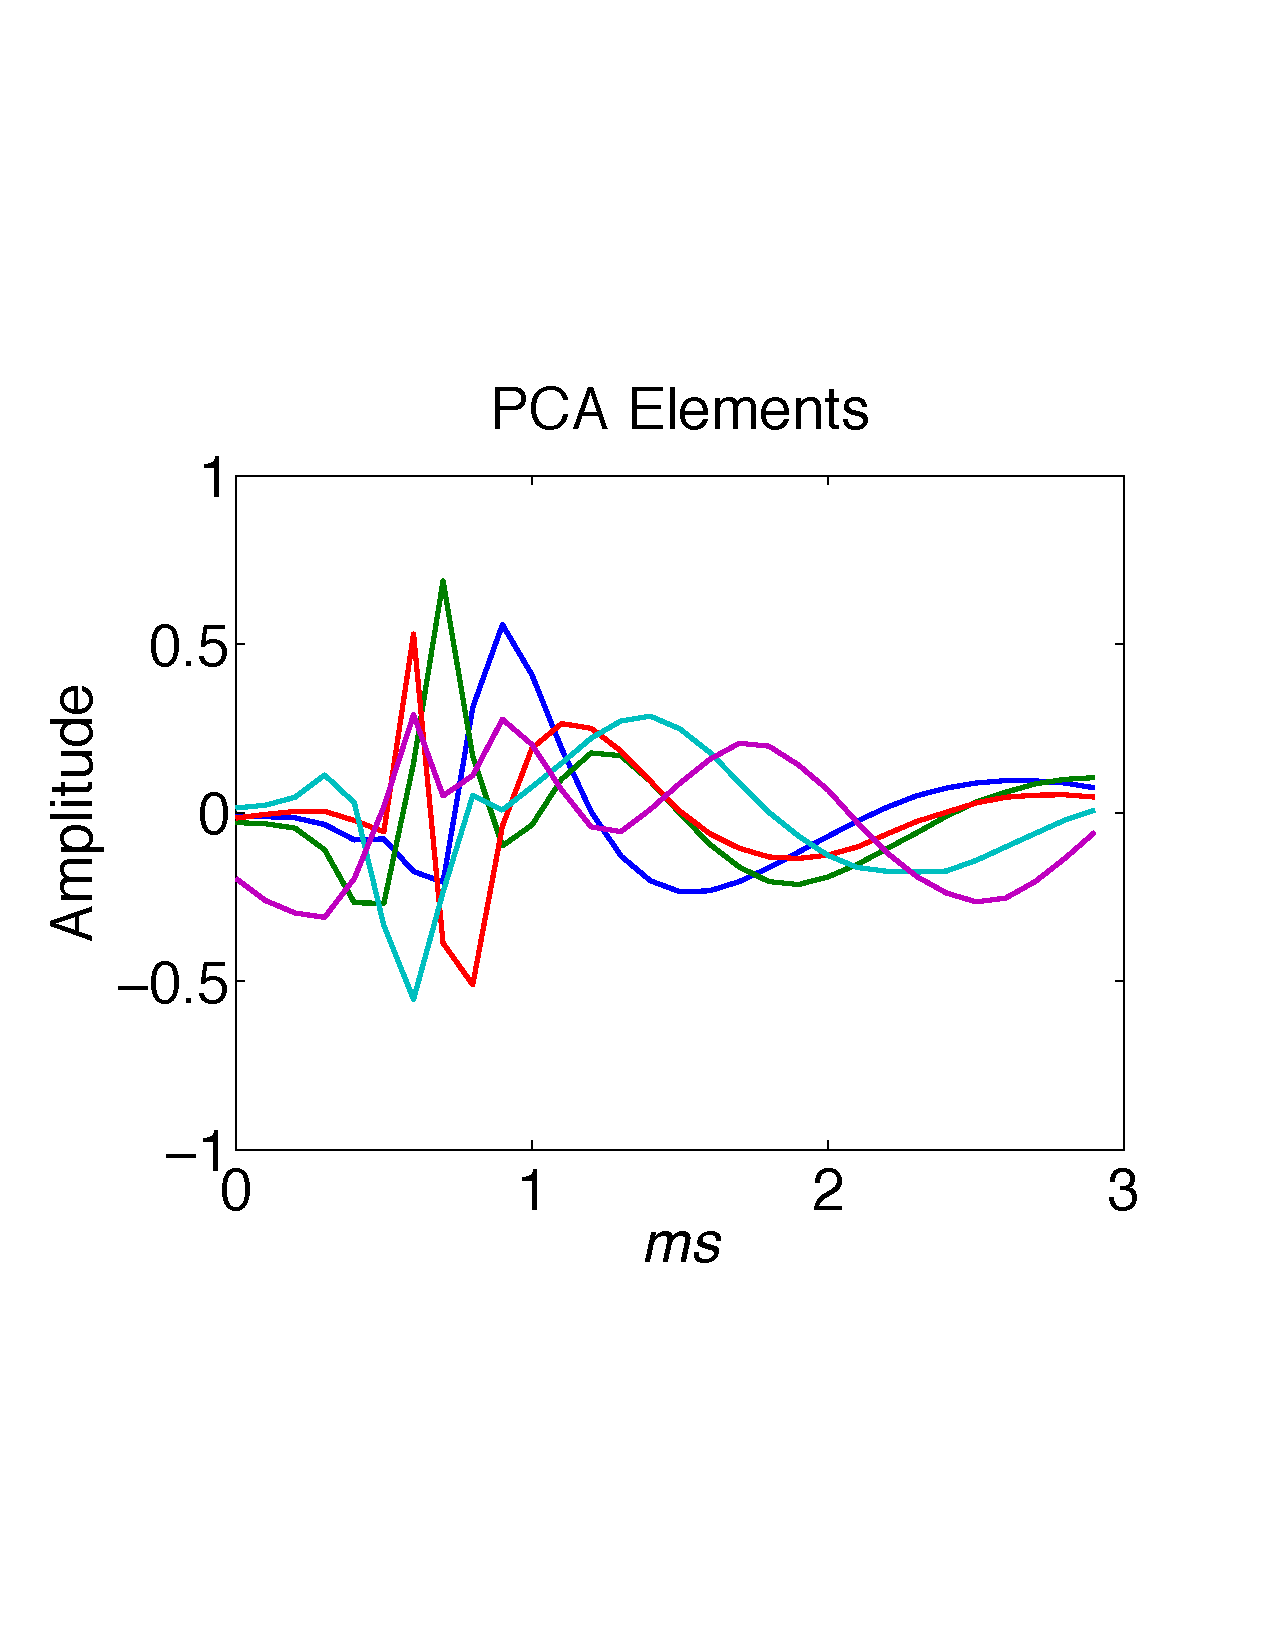
\includegraphics[width=\textwidth]{../figs/new/pcaelements.pdf}
\caption{}
\label{fig:ICold}
\end{subfigure}
\begin{subfigure}[b]{.3\textwidth}
% 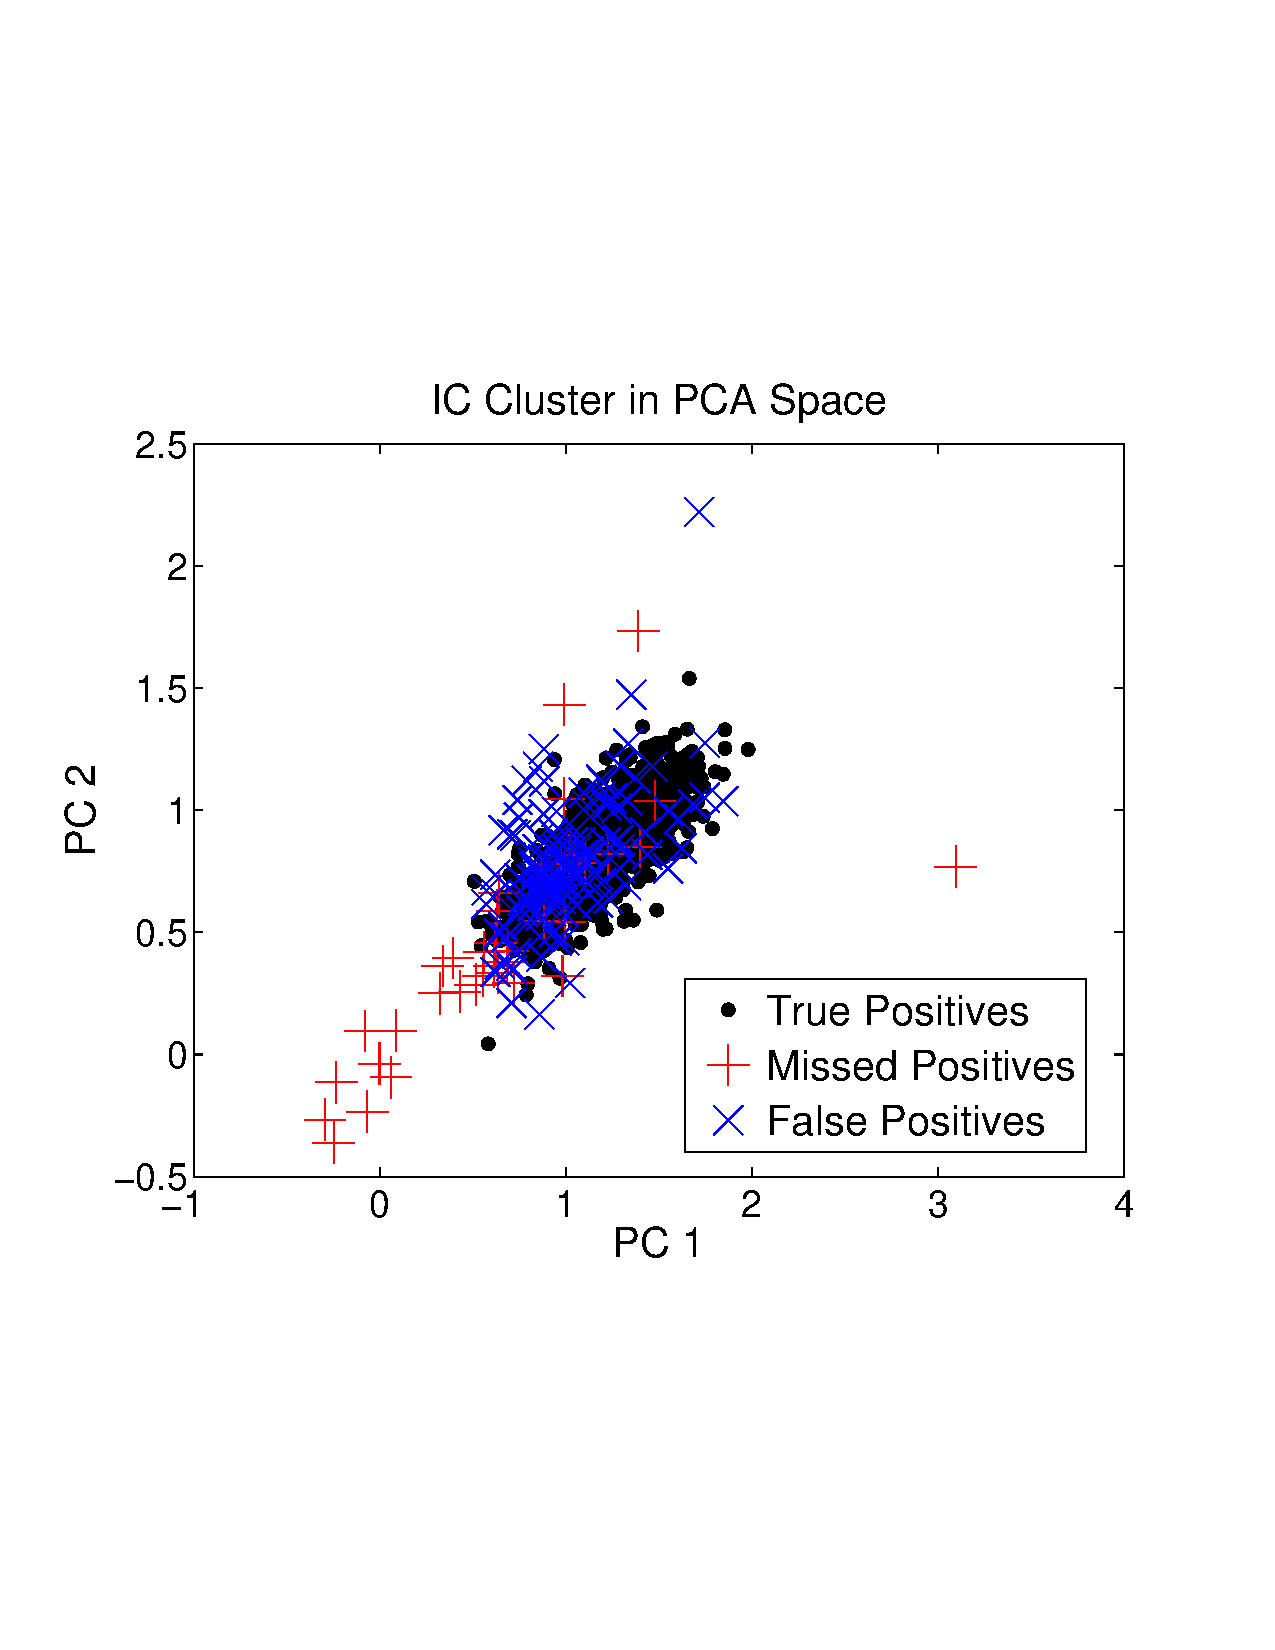
\includegraphics[width=\textwidth]{../figs/new/ICclusteroldpca.pdf}
\caption{}
\label{fig:ICold}
\end{subfigure}
\begin{subfigure}[b]{.3\textwidth}
% 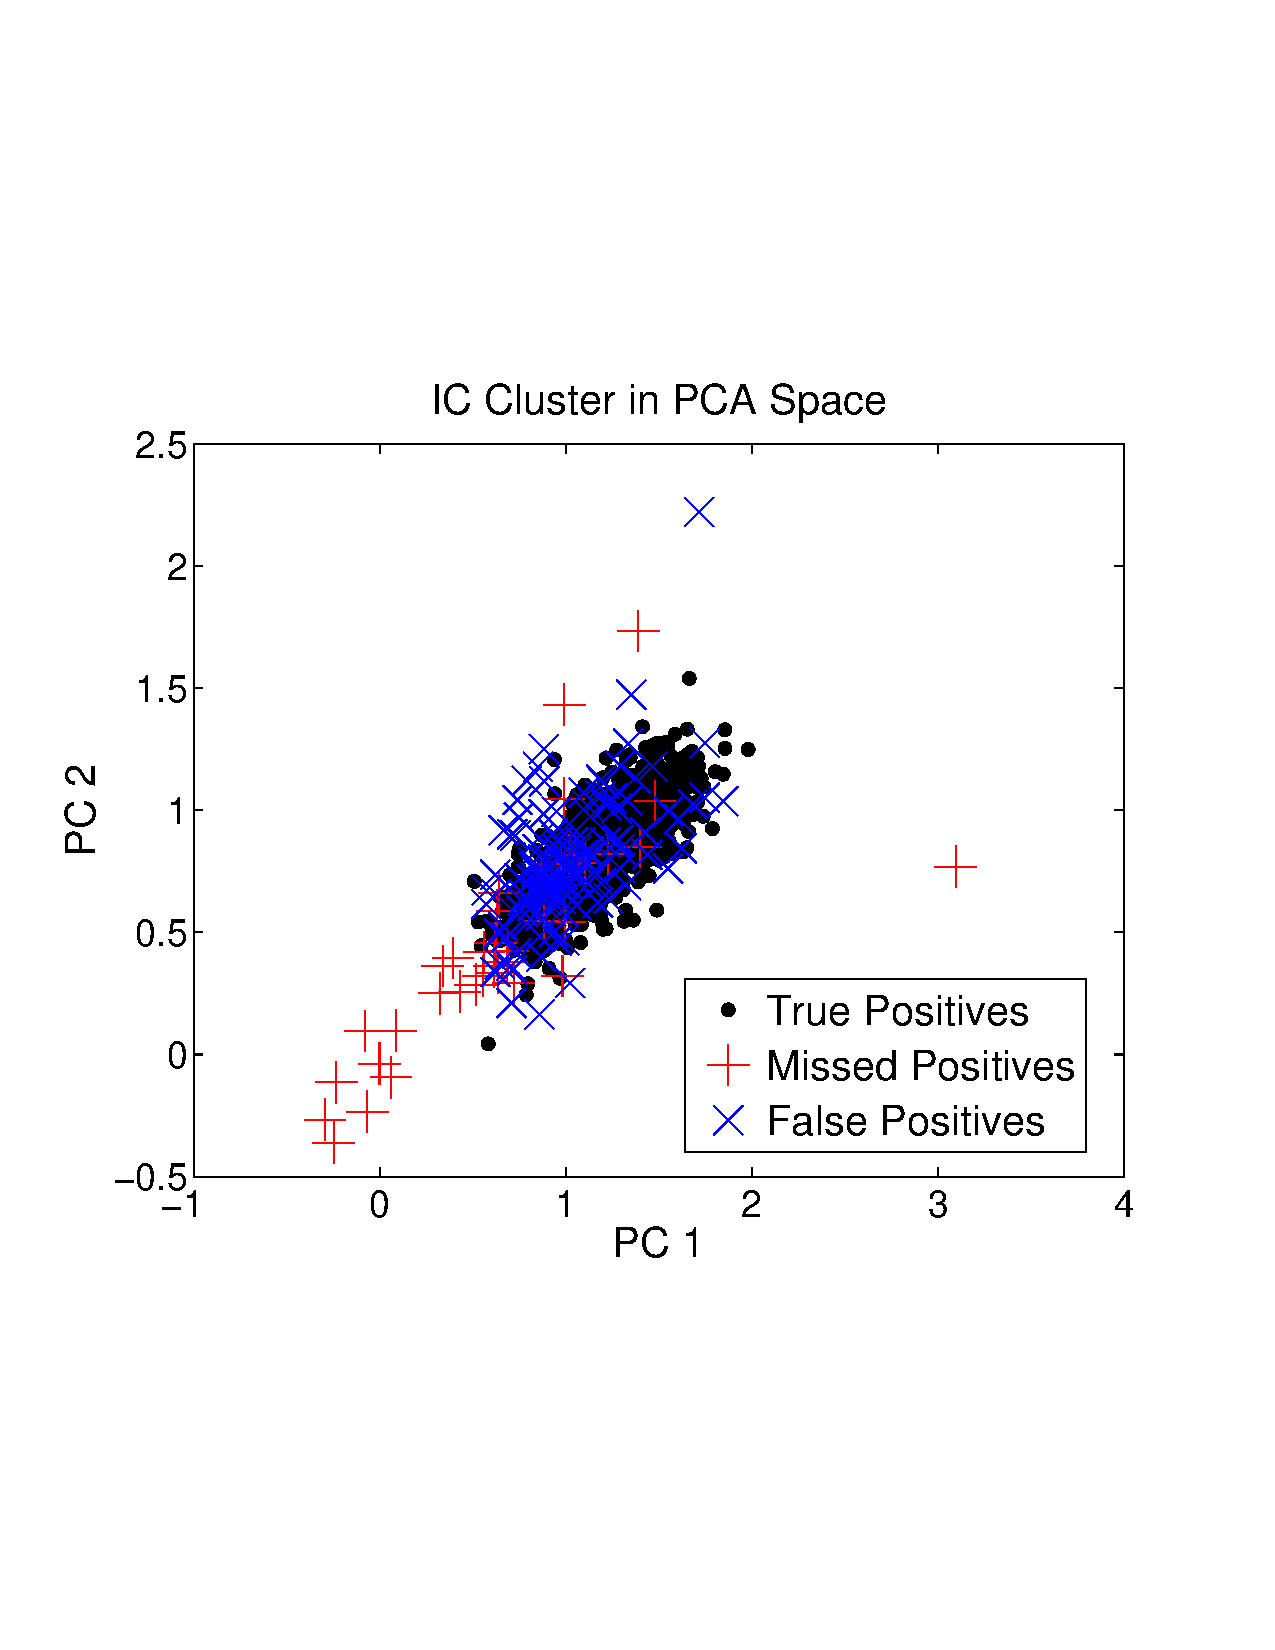
\includegraphics[width=\textwidth]{../figs/new/ICclusteroldpca.pdf}
\caption{}
\label{fig:ICold}
\end{subfigure}
\caption{\jovo{dictionary: (a) from first 5 secs, (b) from all data, (c) spectrum from all data which is cumsum/sum} 
} \label{fig:timing}
\end{figure}
\end{center}

\begin{figure}[htbp]
	\centering
		% 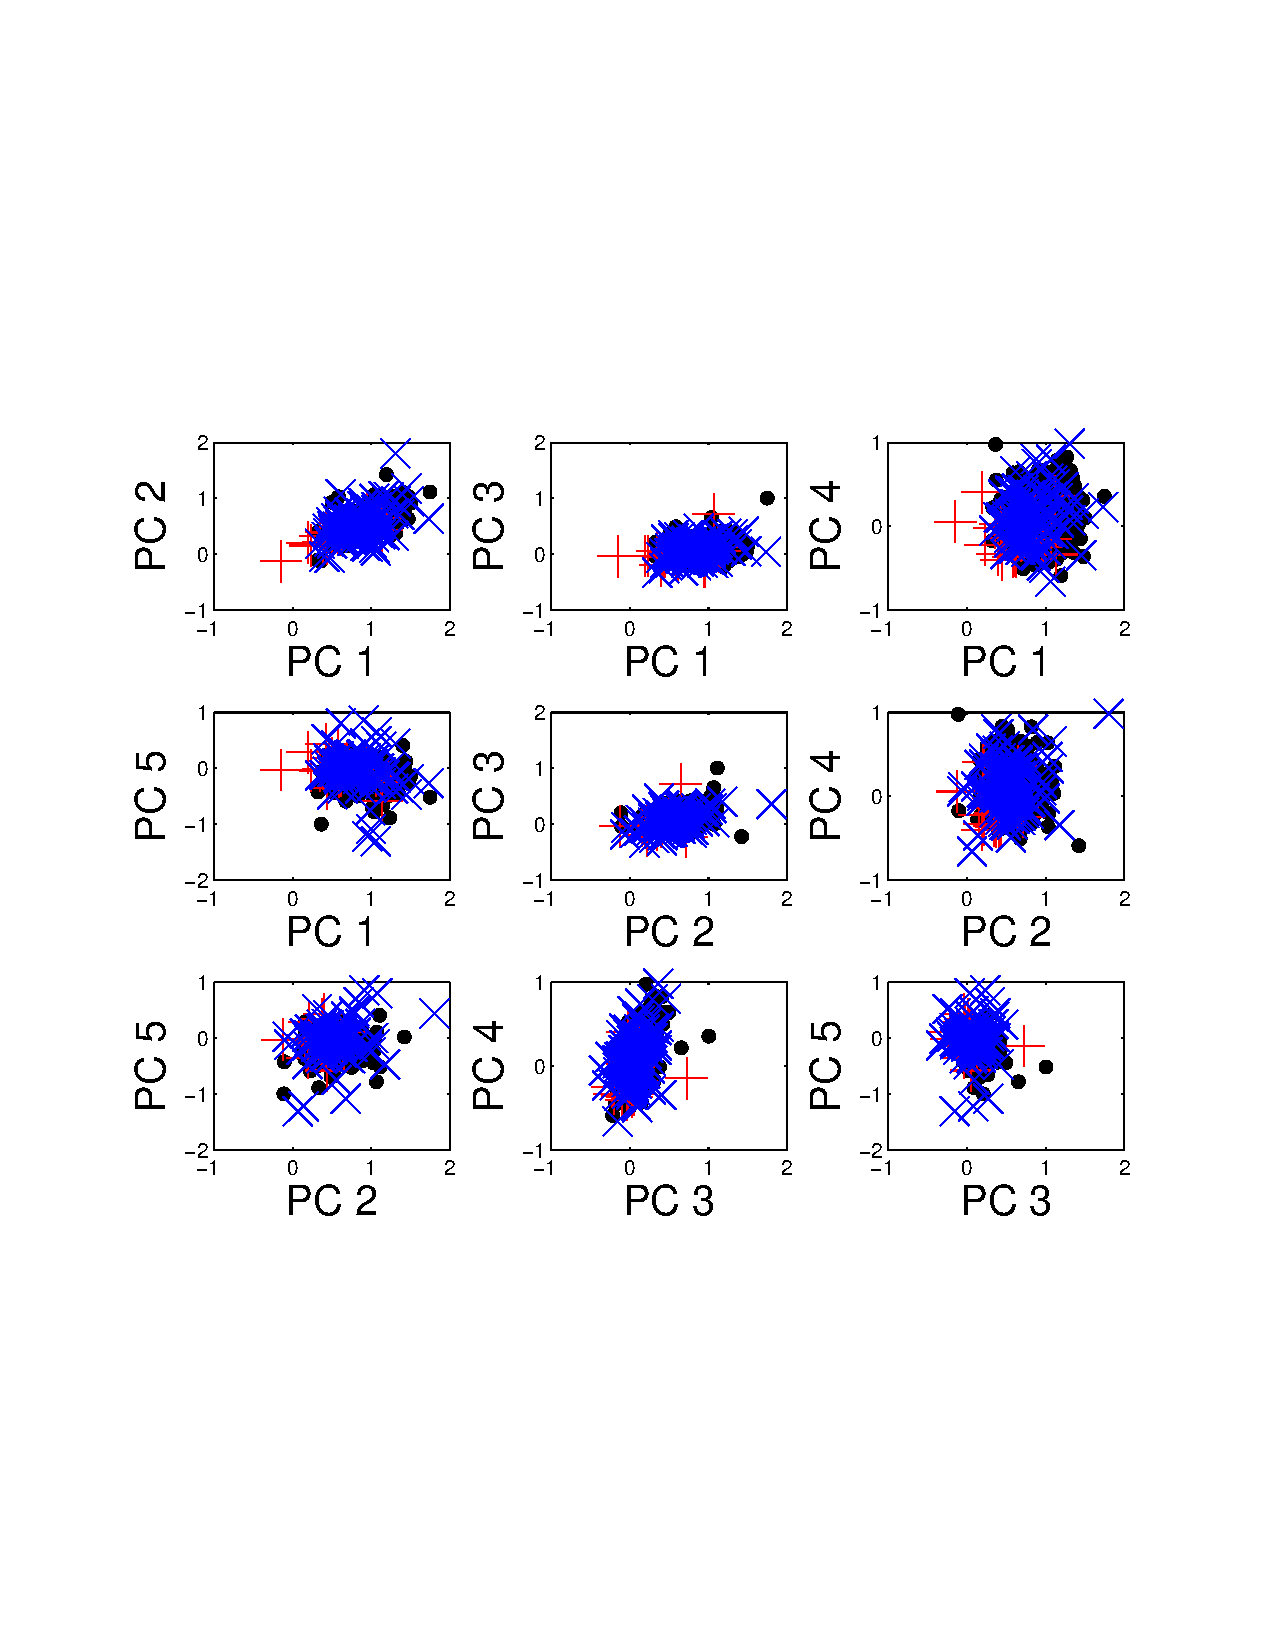
\includegraphics[height=3in]{../figs/new/pairs.pdf}
	\caption{(a) This shows the average number of true positives versus the average number of false positives in the intracellular cluster for 2 minute segments of the 4 minutes of the experiment.  \smug\ does better than    \jovo{let's make the symbols different for the different methods.  also, let's make the axes in terms of percentages, rather than raw numbers.} }
	\label{fig:pairs}
\end{figure}


\begin{figure}[htbp]
	\centering
		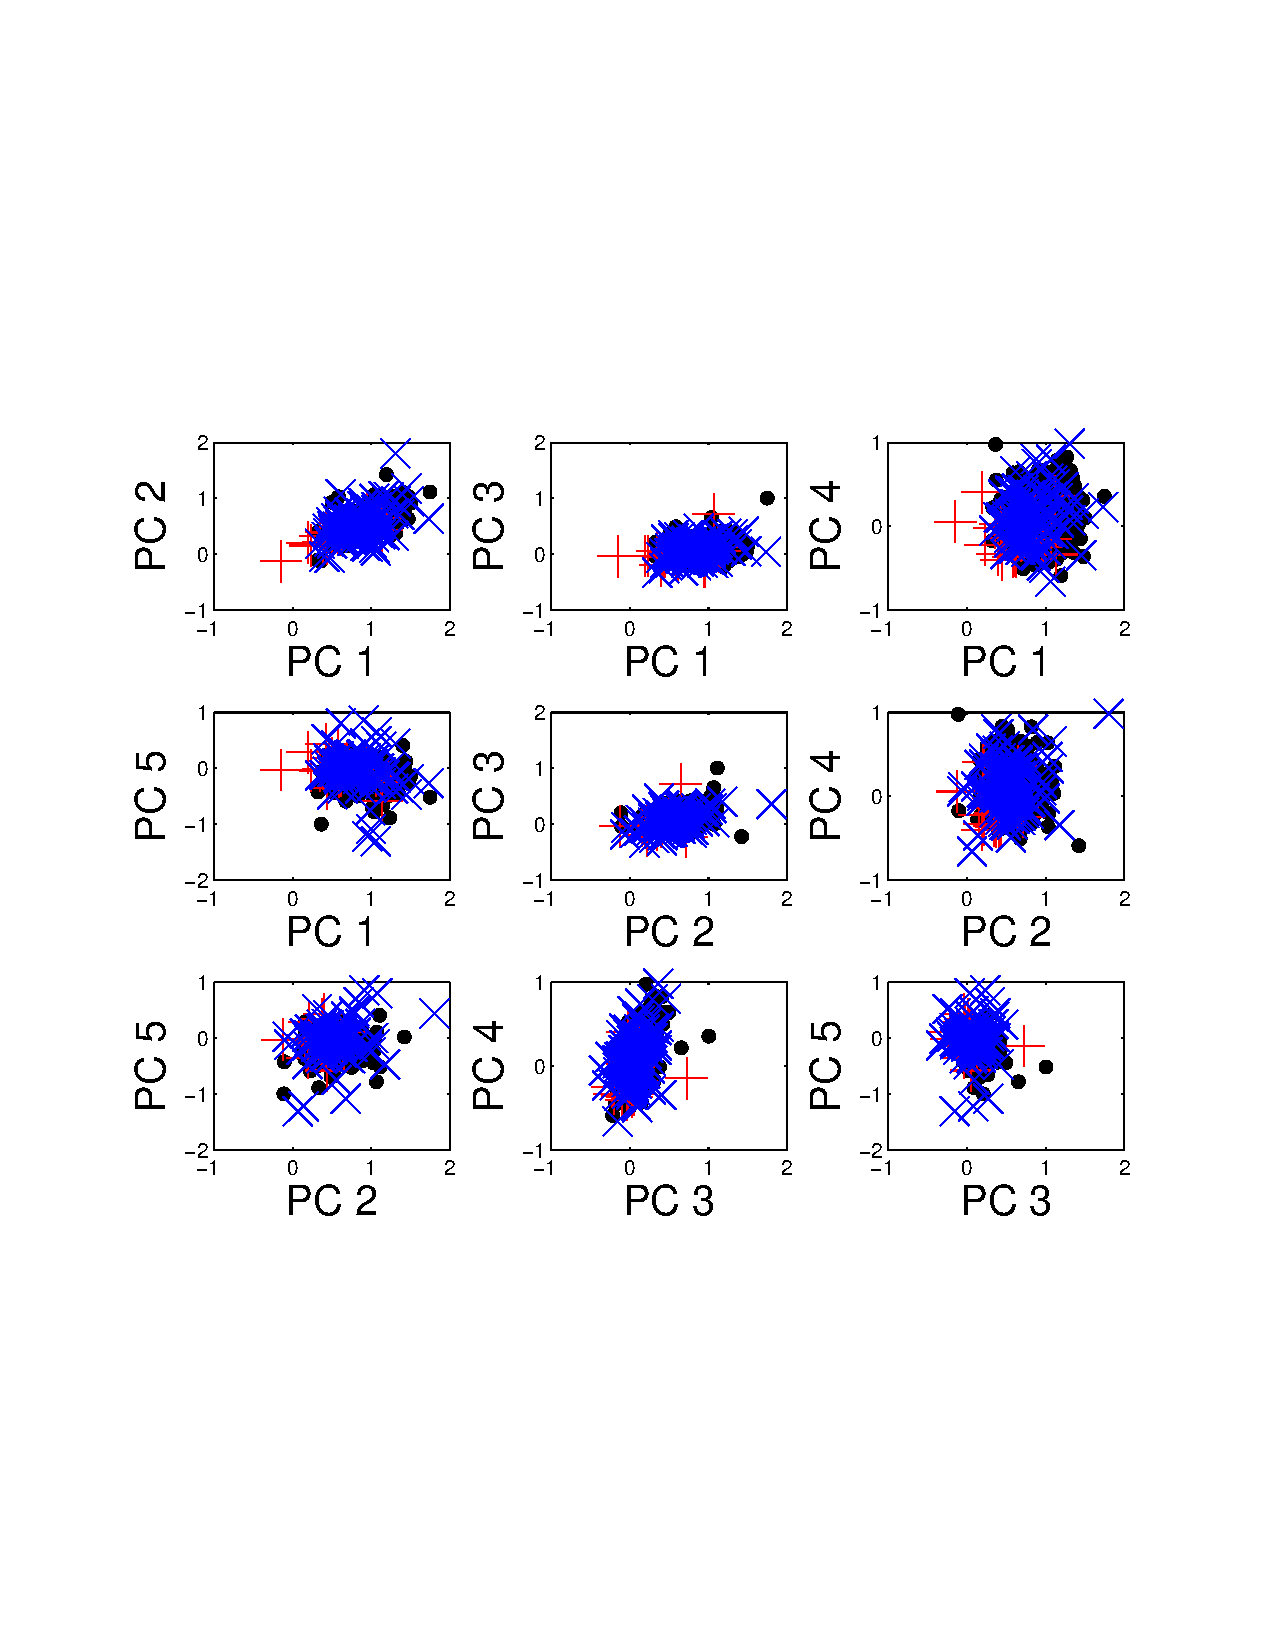
\includegraphics[height=3in]{../figs/new/pairs.pdf}
	\caption{caption}
	\label{fig:pairs}
\end{figure}



\begin{figure}[htbp]
	\centering
		% 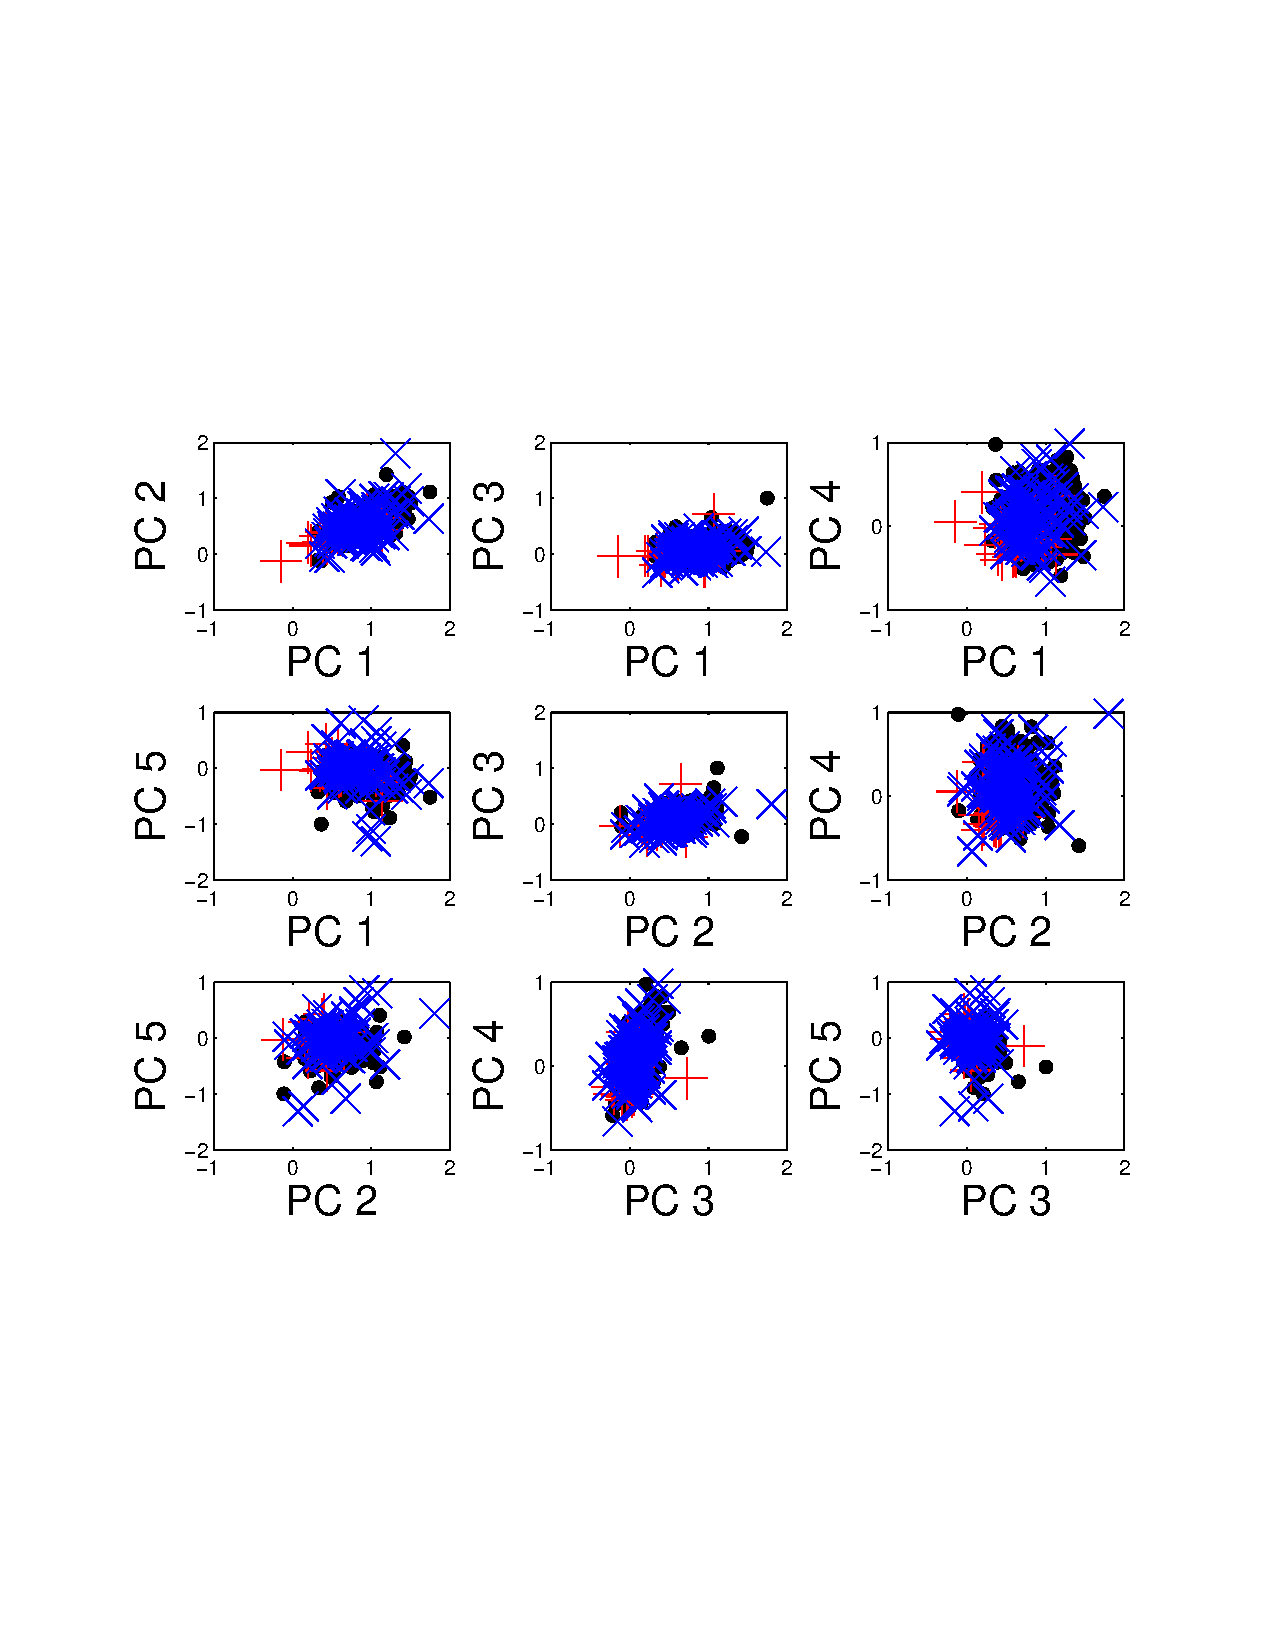
\includegraphics[height=3in]{../figs/new/pairs.pdf}
	\caption{(a) intracellular waveform shape over time (b) and in PC space.}
	\label{fig:pairs}
\end{figure}



\begin{center}
\begin{figure}
\begin{subfigure}[b]{.12\textwidth}
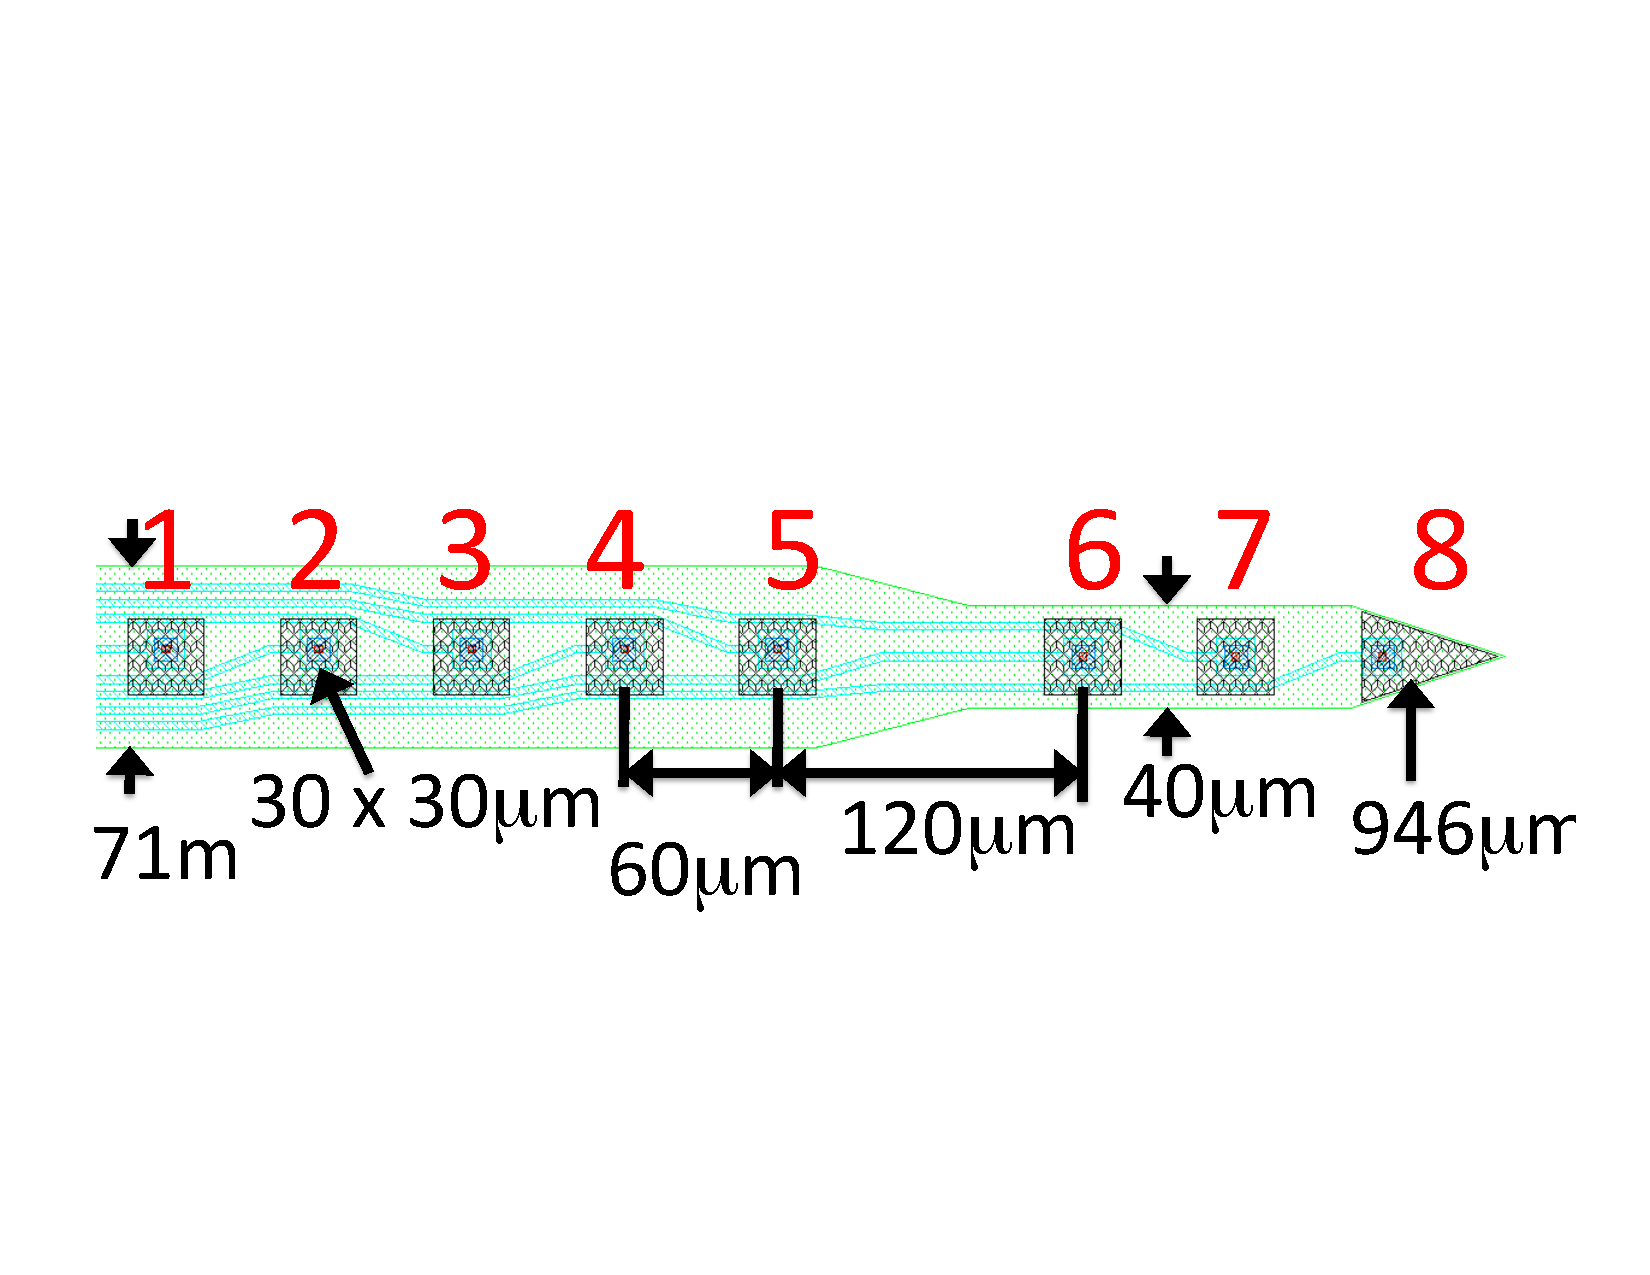
\includegraphics[width=0.8\textwidth]{../figs/8dev}
\caption{}
\label{8dev}
\end{subfigure}
\begin{subfigure}[b]{.28\textwidth}
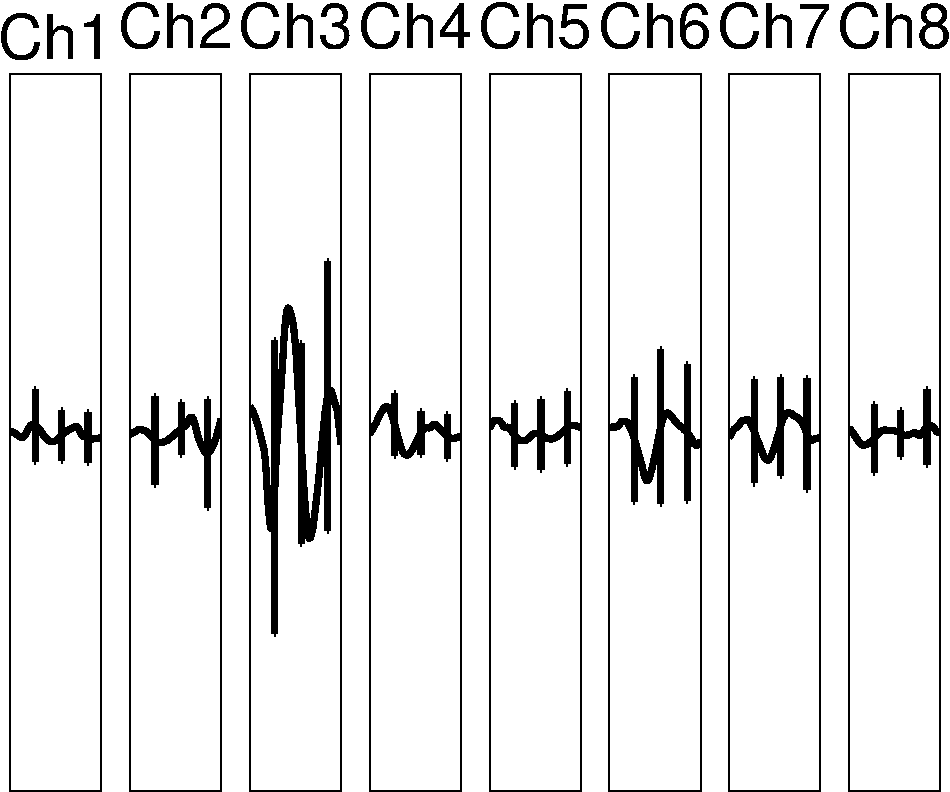
\includegraphics[width=\textwidth]{../figs/8devim/clus3}
\caption{}
\label{ex81}
\end{subfigure}
\begin{subfigure}[b]{.28\textwidth}
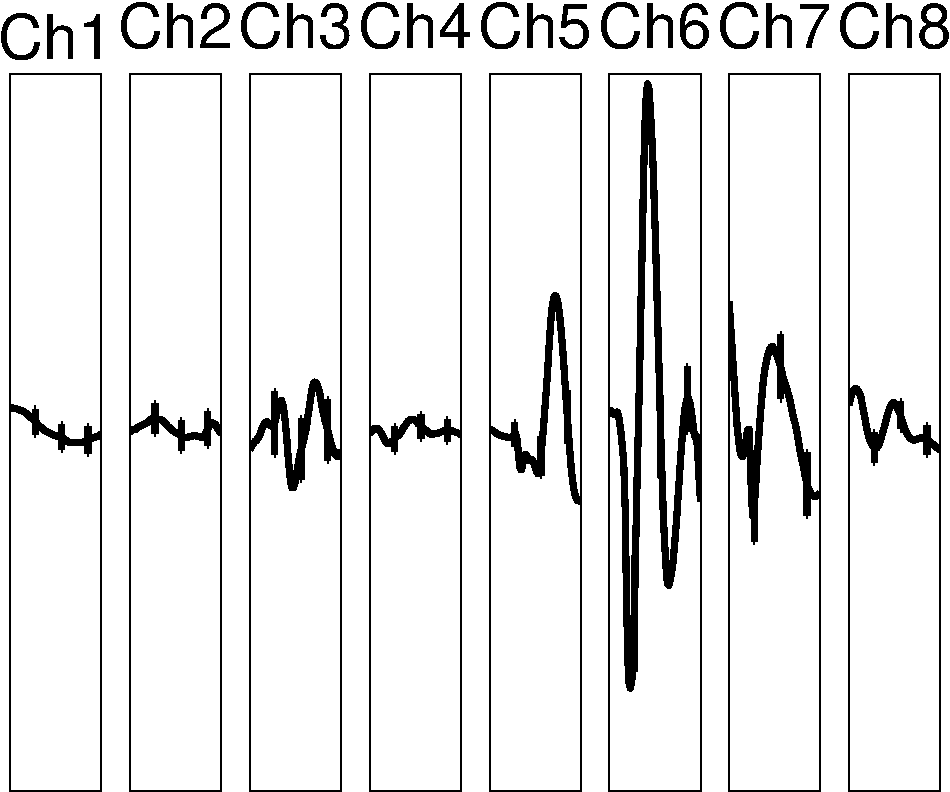
\includegraphics[width=\textwidth]{../figs/8devim/clus9}
\caption{}
\label{ex82}
\end{subfigure}
\begin{subfigure}[b]{.28\textwidth}
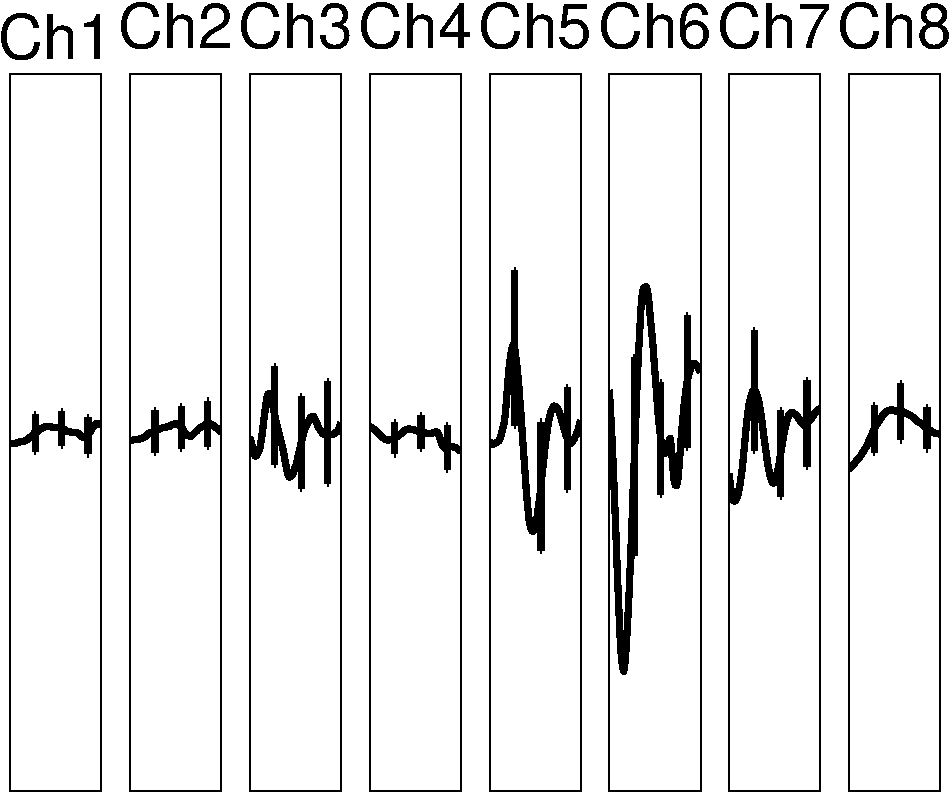
\includegraphics[width=\textwidth]{../figs/8devim/clus6}
\caption{}
\label{ex83}
\end{subfigure}
\caption{
\smug\ multielectrode performance.
(a) 8 electrode device showing local proximity of electrodes with channel indexes in large, red numbers. (b,c,d) Top three most prevalent waveforms.  Each waveform shape is 2 ms long.
} \label{sfig:8}
\end{figure}
\end{center}



\begin{center}
\begin{figure}[h!]
\begin{subfigure}[b]{.5\textwidth}
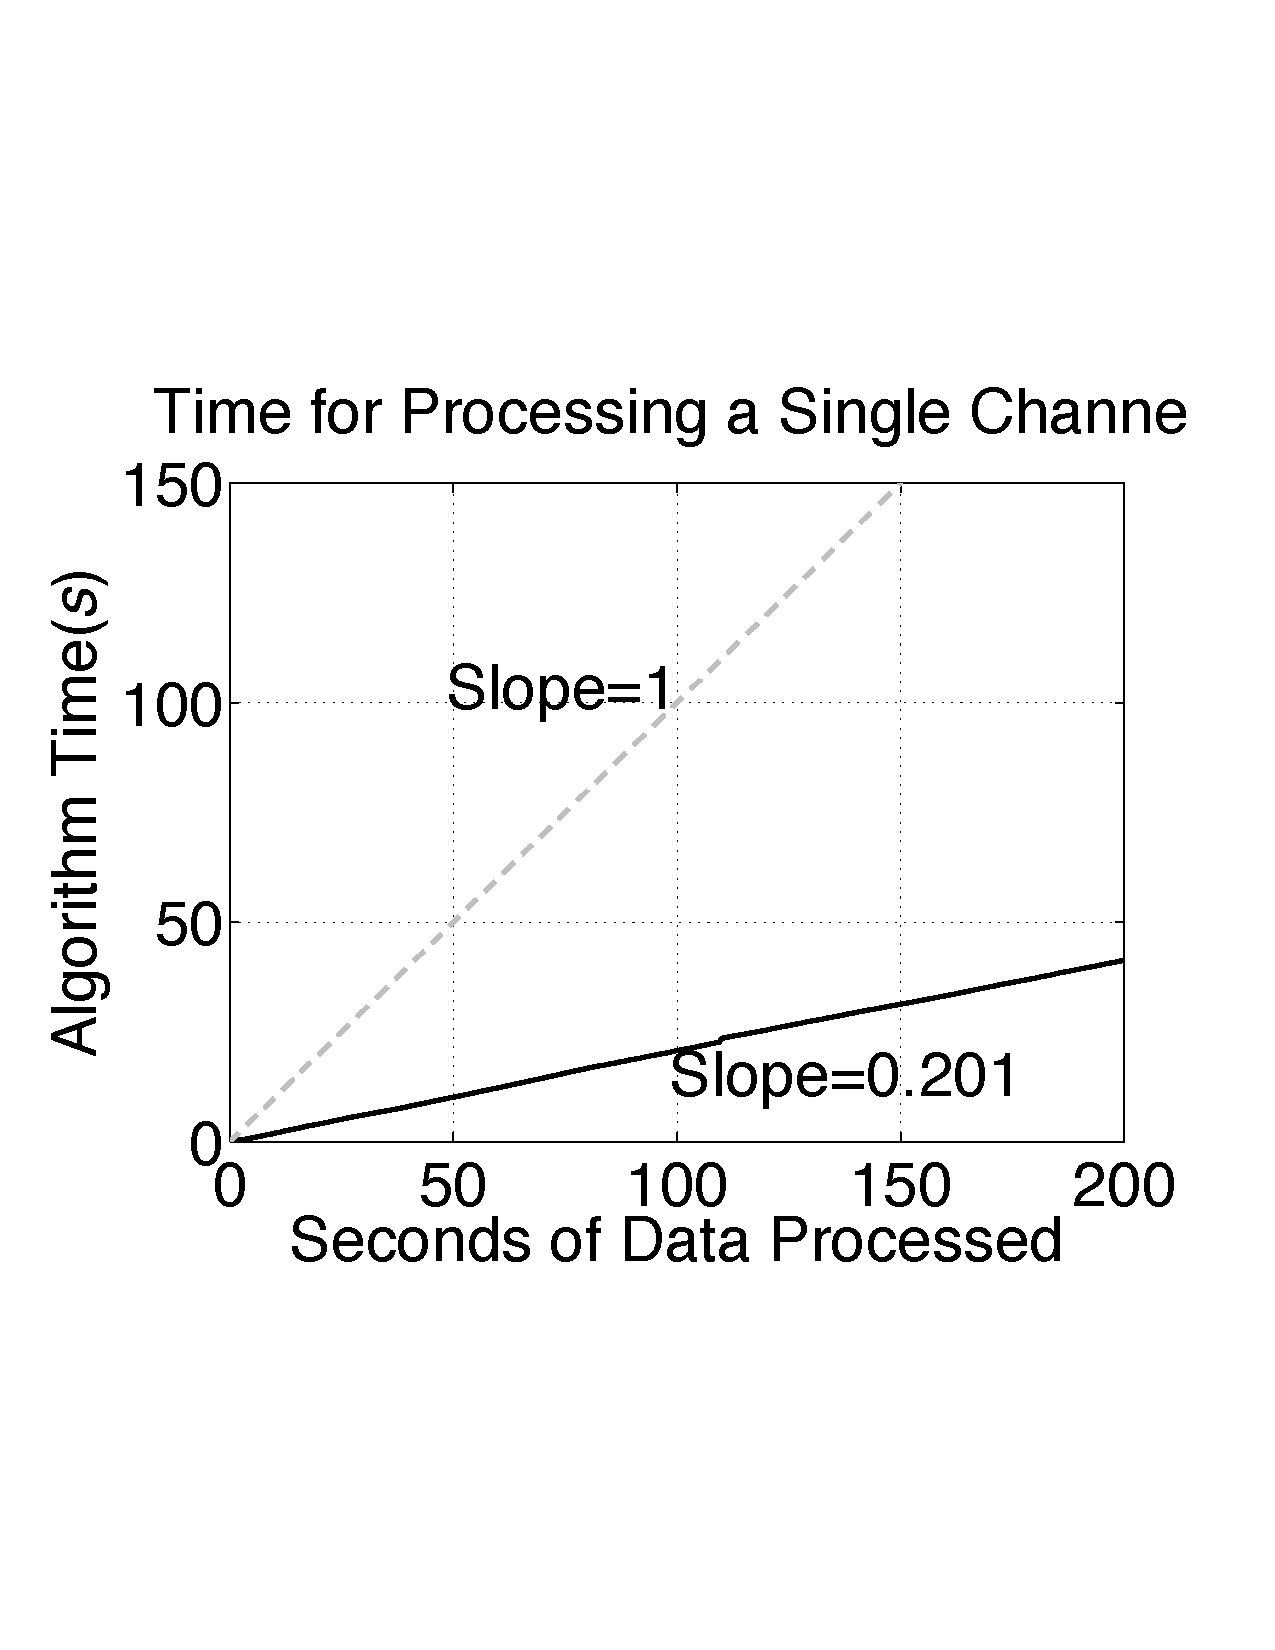
\includegraphics[width=\textwidth]{../figs/new/timingsinglechannel.pdf}
\caption{}
\label{fig:ICold}
\end{subfigure}
\begin{subfigure}[b]{.5\textwidth}
% 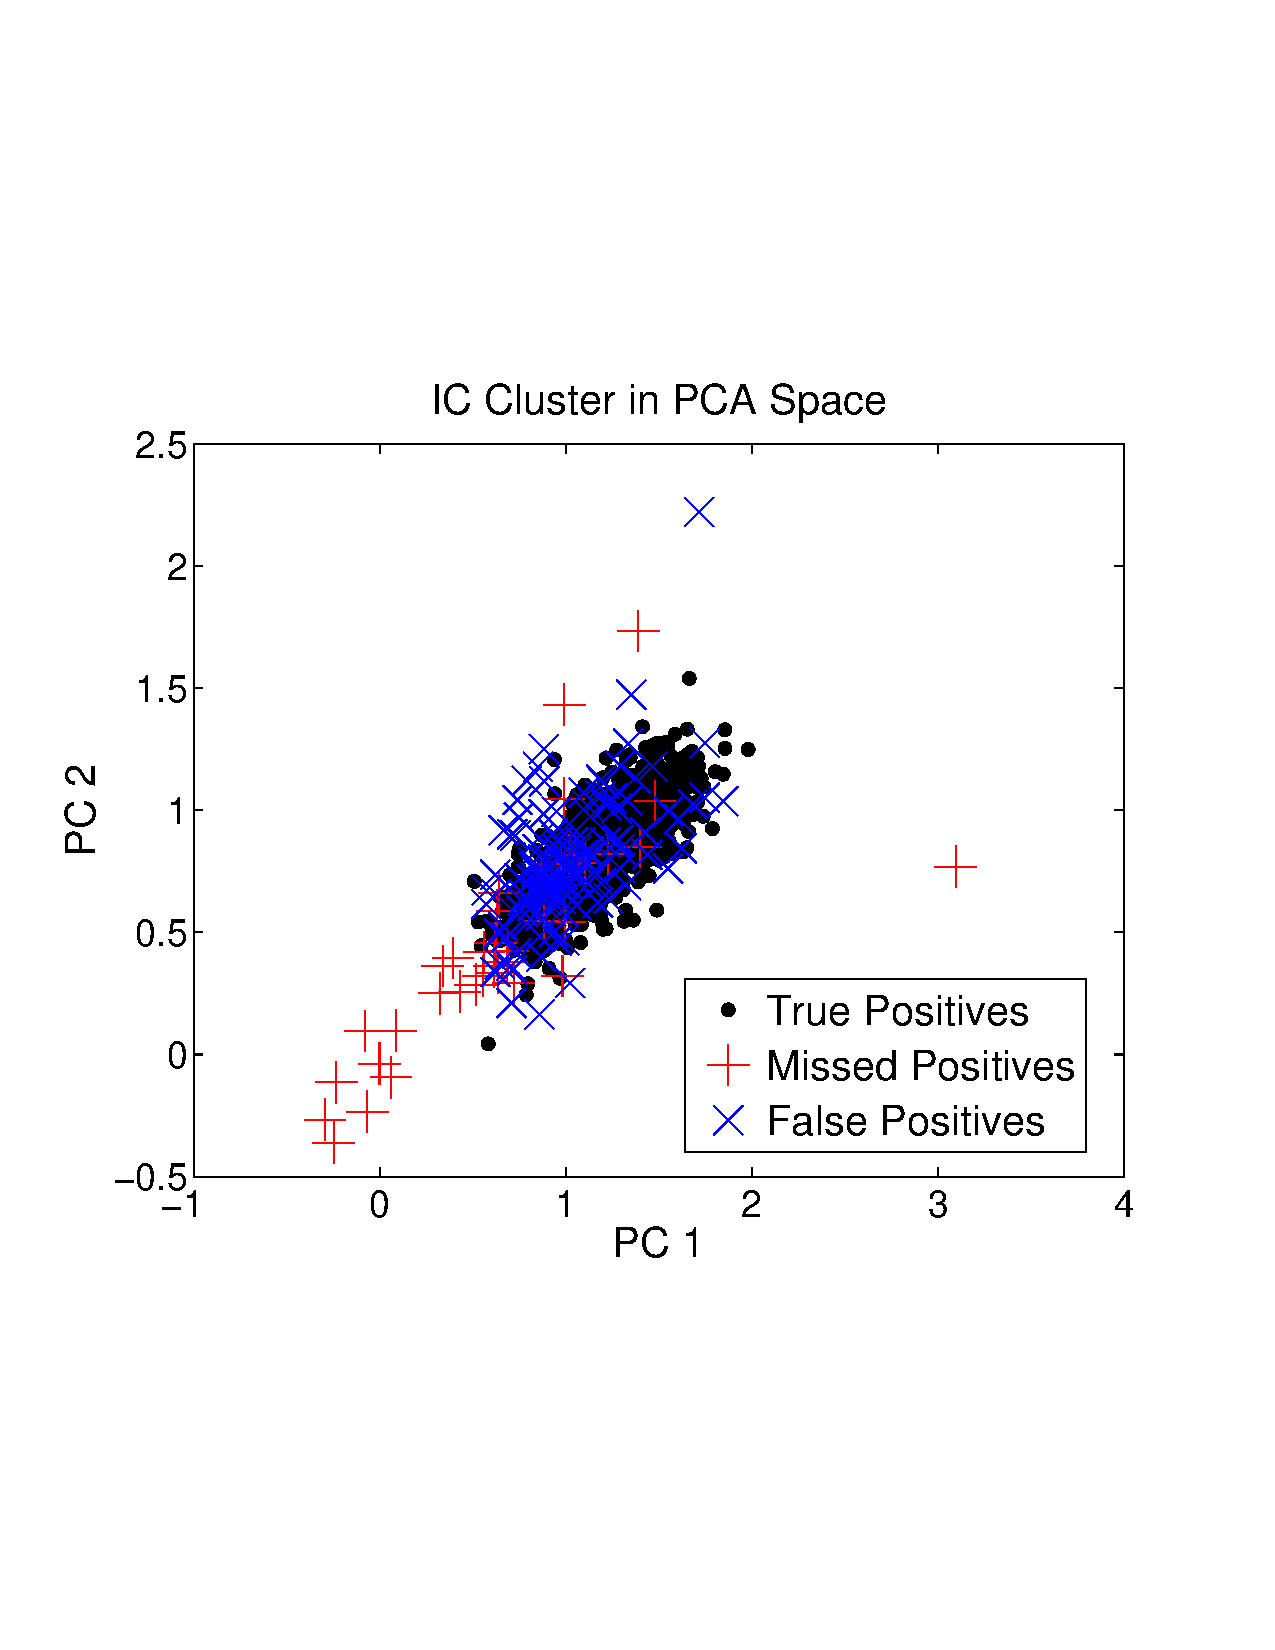
\includegraphics[width=\textwidth]{../figs/new/ICclusteroldpca.pdf}
\caption{}
\label{fig:ICold}
\end{subfigure}
\caption{\jovo{timing plots: (a) line (can we put a line on there for 4 channels too?), (b) notched boxplots. } 
} \label{fig:timing}
\end{figure}
\end{center}

